\documentclass[a4paper]{oblivoir}

\title{쟤료공학개론 과제1}
\author{2018-12432, Electrical and Computer Engineering department, ParkJeonghyun}
\date{9/19/2023}

\newcommand{\be}{\begin{equation}}
\newcommand{\ee}{\end{equation}}

\usepackage{fapapersize}
\usepackage{amsmath}
\usepackage{MnSymbol}
\usepackage{wasysym}
\usepackage{graphicx}
\usepackage{caption}
\usepackage{subfig}
\usepackage{hyperref}
\usepackage{cite}
\usepackage{dtk-logos}
\usepackage{physics}
\usepackage{tikz}
\usetikzlibrary{decorations.markings, positioning}
\usepackage{dtk-logos}
\usepackage{fancyvrb}
\usepackage{array} 

\usefapapersize{ 210mm, 297mm, 15mm, 15mm, 15mm, 15mm}
\DeclareGraphicsExtensions{.pdf, .png, .jpg}

\renewcommand{\figurename}{Figure}

\begin{document}

\maketitle
\section{Problem 1}
\subsection{1}
\indent $E_{N}$을 미분하면 아래와 같다.
\begin{align}
	\frac{dE_{N}}{dr} &= \frac{A}{r^{2}} - \frac{nB}{r^{n+1}} = 0
\end{align}
평형점에서는 해당 미분값이 0이므로 해당 $r_{0}$라고하자.
\subsection{2}
\begin{align}
	\frac{A}{r_{0}^{2}} - \frac{nB}{r_{0}^{n+1}} &= 0\\
	Ar_{0}^{n-1}&=nB\\
	r_{0} &= \left(\frac{nB}{A}\right)^{\frac{1}{n-1}}\label{eq:r0}
\end{align}
\subsection{3}
$r_{0}$를 $E_{N}$에 대입하면 아래와 같다.
\begin{align}
	E_{0} &= -\frac{A}{r_{0}} + \frac{B}{r_{0}^{n}}\\
	&= -\left( 1- \frac{1}{n} \right)\frac{A}{r_{0}}\\
	&= -\left( 1- \frac{1}{n} \right)A\left(\frac{A}{nB}\right)^{\frac{1}{n-1}}\label{eq:E0}
\end{align}


\section{Problem 2}
\subsection{1}
에너지 곡선을 그리면 Fig.\ref{fig:P2_1}와 같다.

\begin{figure}[htbp]
	\centerline{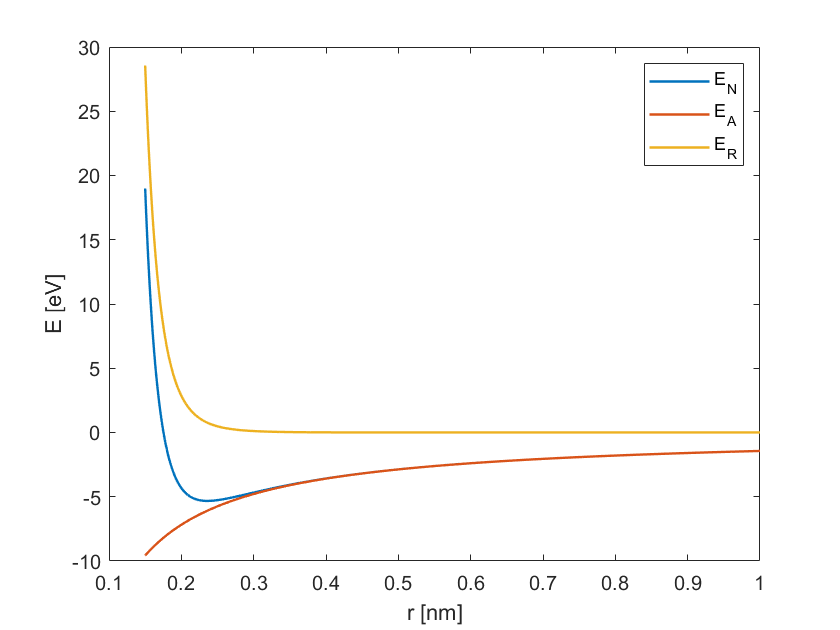
\includegraphics[width = 0.6\linewidth]{P2_1.png}}% Here is how to import EPS art
	\caption{\label{fig:P2_1}에너지 그래프}
\end{figure}
\subsection{2}
에너지 곡선에서 최저점을 찾으면 Fig.\ref{fig:P2_2}와 같다.

\begin{figure}[htbp]
	\centerline{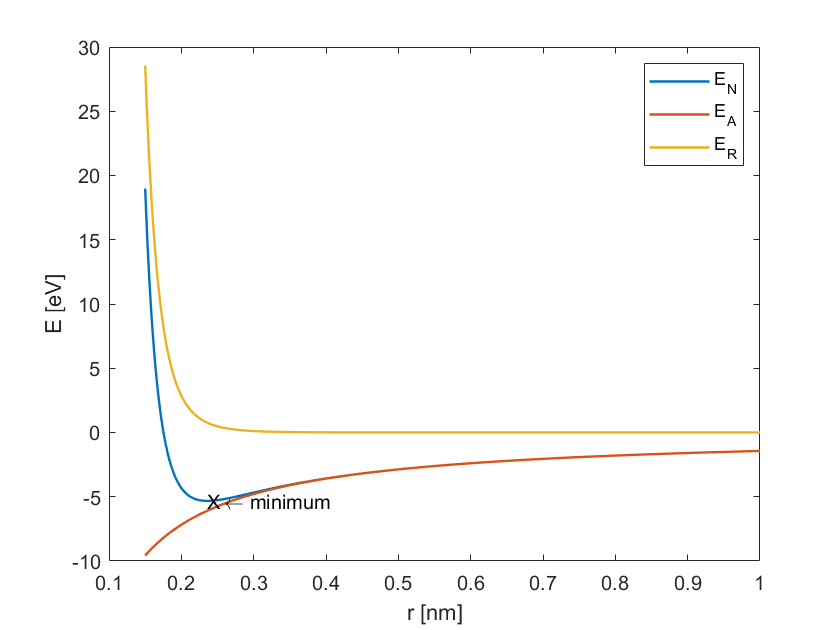
\includegraphics[width = 0.6\linewidth]{P2_2.png}}% Here is how to import EPS art
	\caption{\label{fig:P2_2}에너지 그래프}
\end{figure}


\subsection{3}
(\ref{eq:r0}) 와 (\ref{eq:E0})을 이용하여 계산하면 아래와 같다.

\begin{align}
	r_{0} &= 0.2360 nm\\
	E_{0} &= -5.3240 eV
\end{align}

해당 값은 그래프에서 찾은 위치와 일치한다.

\section{Problem 3}
\subsection{1}
이온화 정도는 아래의 식과 같다.
\begin{align}
	Ionic &= 1 - \exp\left( - \frac{1}{4}|X_{A}-X_{B}|^{2} \right)\\
	&=1 - \exp\left( - \frac{1}{4}|1.6-1.5|^{2} \right)\\
	&= 0.0025
\end{align}

\subsection{2}
Ionic character가 $0.5$보다 충분히 작으므로 공유결합이 주를 이룰 것이다.


\section{Problem 4}
수소는 전기음성도가 $2.20$, 플루오린은 $3.98$, 염소는  $3.16$의 전기음성도를 가진다. 따라서 $HF$, $HCl$은 모두 permanent한 dipole moment를 가진다. 염소의 크기가 더 커 fluctuating하는 dipole에 의해 발생하는 힘은 더 크지만 $HF$의 전기음성도 차이가 더 커 더 큰 permanent dipole을 형성하고 강한 수소 결합을 하게 되므로 $HF$의 끓는점이 더 높다.

\section{Problem 5}
Solid xenon은 비활성 기체의 고체 형태이므로 반데르발스 힘이 주로 작용할 것이다. $CaF_{2}$의 경우 물질을 이루는 원소의 전기음성도 차이가 크므로 $Ca^{2+}$, $F^{-}$가 이온 결합을 하게 될 것이다. $Cu$의 경우 금속 원소에 해당하므로 금속 결합이 주를 이룰 것이다. $CdTe$의 경우 각각 $1.69$, $2.1$의 전기음성도를 가지므로 ionic character는 $1 - \exp\left( - \frac{1}{4}|1.69-2.1|^{2} \right)$ $=4\%$에 해당한다. 따라서 공유결합이 주를 이룬다. 고무의 분자식은 $[(CH_{2})C_{2}H(CH_{3})(CH_{2})]_{n}$으로 탄소와 수소사이의 전기음성도 차이로 인해 분자들간에 수소결합을 이루게 된다. 하지만 원자들 사이에서는 공유결합을 하게 된다. 텅스텐은 금속원소이므로 금속결합을 하게 된다.

\end{document}